
\graphicspath{ {mainmatter/Serafin_2004/} }
\title*{2004: Toward a Generalized Friction Controller: From the Bowed
String to Unusual Musical Instruments}

\titlerunning{A Generalized Friction Controller}

\author{Stefania Serafin and Diana Young}
\authorrunning{Serafin and Young}

%\institute{Stefania Serafin \at, \email{}
%\and Diana Young \at, \email{}}
%

%
\maketitle

\abstract*{
We present case studies of unusual instruments that share the same excitation mechanism as that of the bowed string. The musical saw, Tibetan singing bow, glass harmonica, and bowed cymbal all produce sound by rubbing a hard object on the surface of the instrument. For each, we discuss the design of its physical model and present a means for expressively controlling it. Finally, we propose a new kind of generalized friction controller to be used in all these examples.}

\section{Introduction}
Playability of physical models is an area of increasing interest in recent years. As the synthesis techniques have become suitably refined to compare favorably with their real instrument counterparts, access to the many musical possibilities they offer has remained somewhat limited from the standpoint of the performer. That is, though they provide ample material for use in new compositions \cite{Serafin:2003a}, and even inspire the creation of new compositional techniques and notations \cite{Burtner:2003}, they are still generally quite removed from the easy intuitive control of performers. Only when there are natural and instinctive physical ways of playing the sophisticated models in existence today, will these models emerge as true instruments in spite of their virtual origin. Previously, an ongoing virtual violin project was described \cite{Serafin:2003,Young:2003b}, in which a bowed string controller is used to explore the playability of a violin physical model. Though the violin is an example of a highly sophisticated traditional instrument that requires a very complicated playing technique, it relies on an excitation mechanism that is common to many instruments that may be considered unusual by comparison. This paper addresses the issues of controlling physical models of instruments that possess a friction-based excitation mechanism such as that found in the bow-string interaction and the musical possibilities such control might afford Discussed below are the musical saw, Tibetan singing bowl, glass harmonica, and bowed cymbal. We also propose a new generalized controller for friction driven instruments. This controller is able to drive all the instruments described in this paper, as well as other sonorities which are produced by rubbing dry surfaces.

\begin{figure}[t]
\centering
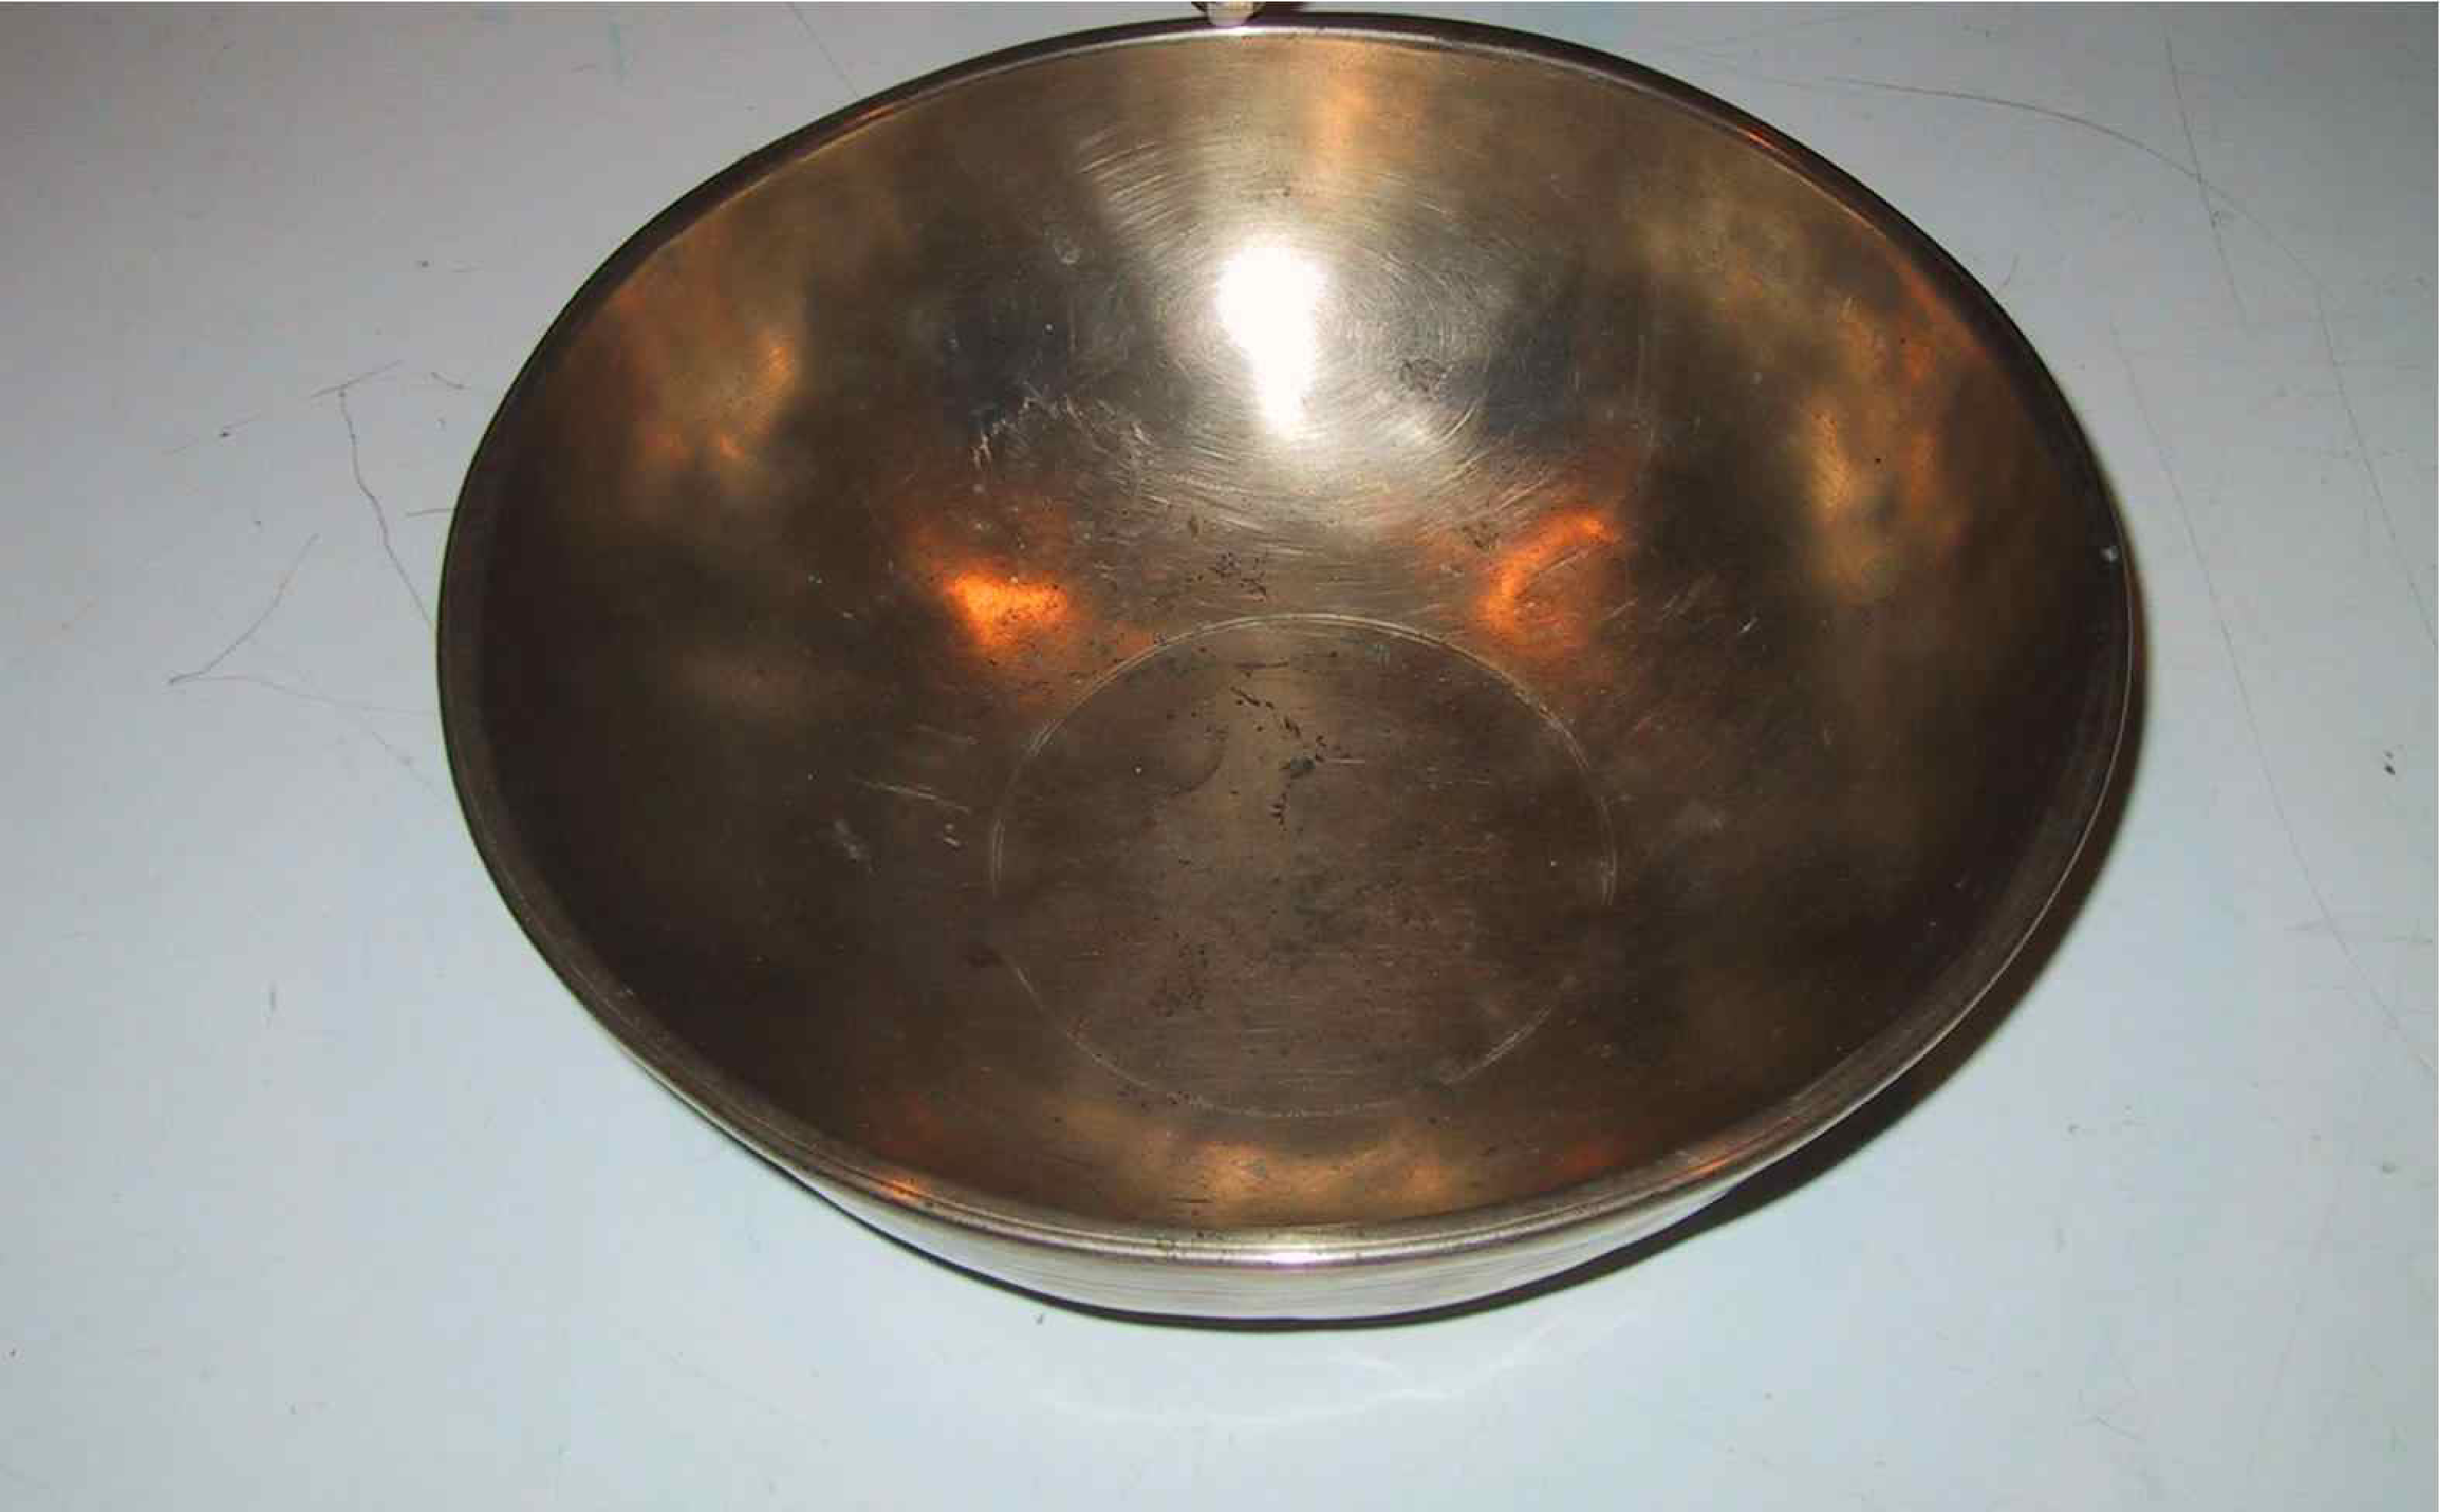
\includegraphics[width=7.8cm]{bowlcarr-eps-converted-to.pdf}
\caption{The Tibetan singing bowl used as a starting point
for the physical model.}
  \label{Serafin:fig:1}
\end{figure}

\section{Tibetan Bowl and Glass Harmonica}

\subsection{The Tibetan Bowl}

Oral tradition dates the singing bowl back to 560-180 B.C. in Tibet. These bowls have been found in temples, monasteries, and meditation halls throughout the world. Singing bowls are said to be made out of five to seven metals such as gold, silver, mercury, copper, iron, metal and tin, each representing a celestial body. Each of these metals is said to produce an individual sound, including partials, and together these sounds produce the exceptional singing sound of the bowl.  Each bowl is hand hammered round to produce beautiful harmonic tones and vibrations. Today they are used in music, relaxation, meditation, and healing.

\subsection{The Glass Harmonica}
Glass harmonicas are musical instruments of two kinds. The first one, invented by Benjamin Franklin, adopts glass bowls turned by a horizontal axle so that one side of the bowl dips into a trough of water. The second one is a combination of wineglasses similar to the ones shown in Figure~\ref{Serafin:fig:2}. Different melodies can be played on a set of tuned glasses (filled with appropriate amounts of water or carefully selected by size), simply by rubbing the edge of the glass with a moist finger. Rubbing rims of glasses in order to produce music became very popular in Europe during the 18th century. Music on glasses has been successfully composed by Mozart, Beethoven, and many others.

\begin{figure}[t]
\centering
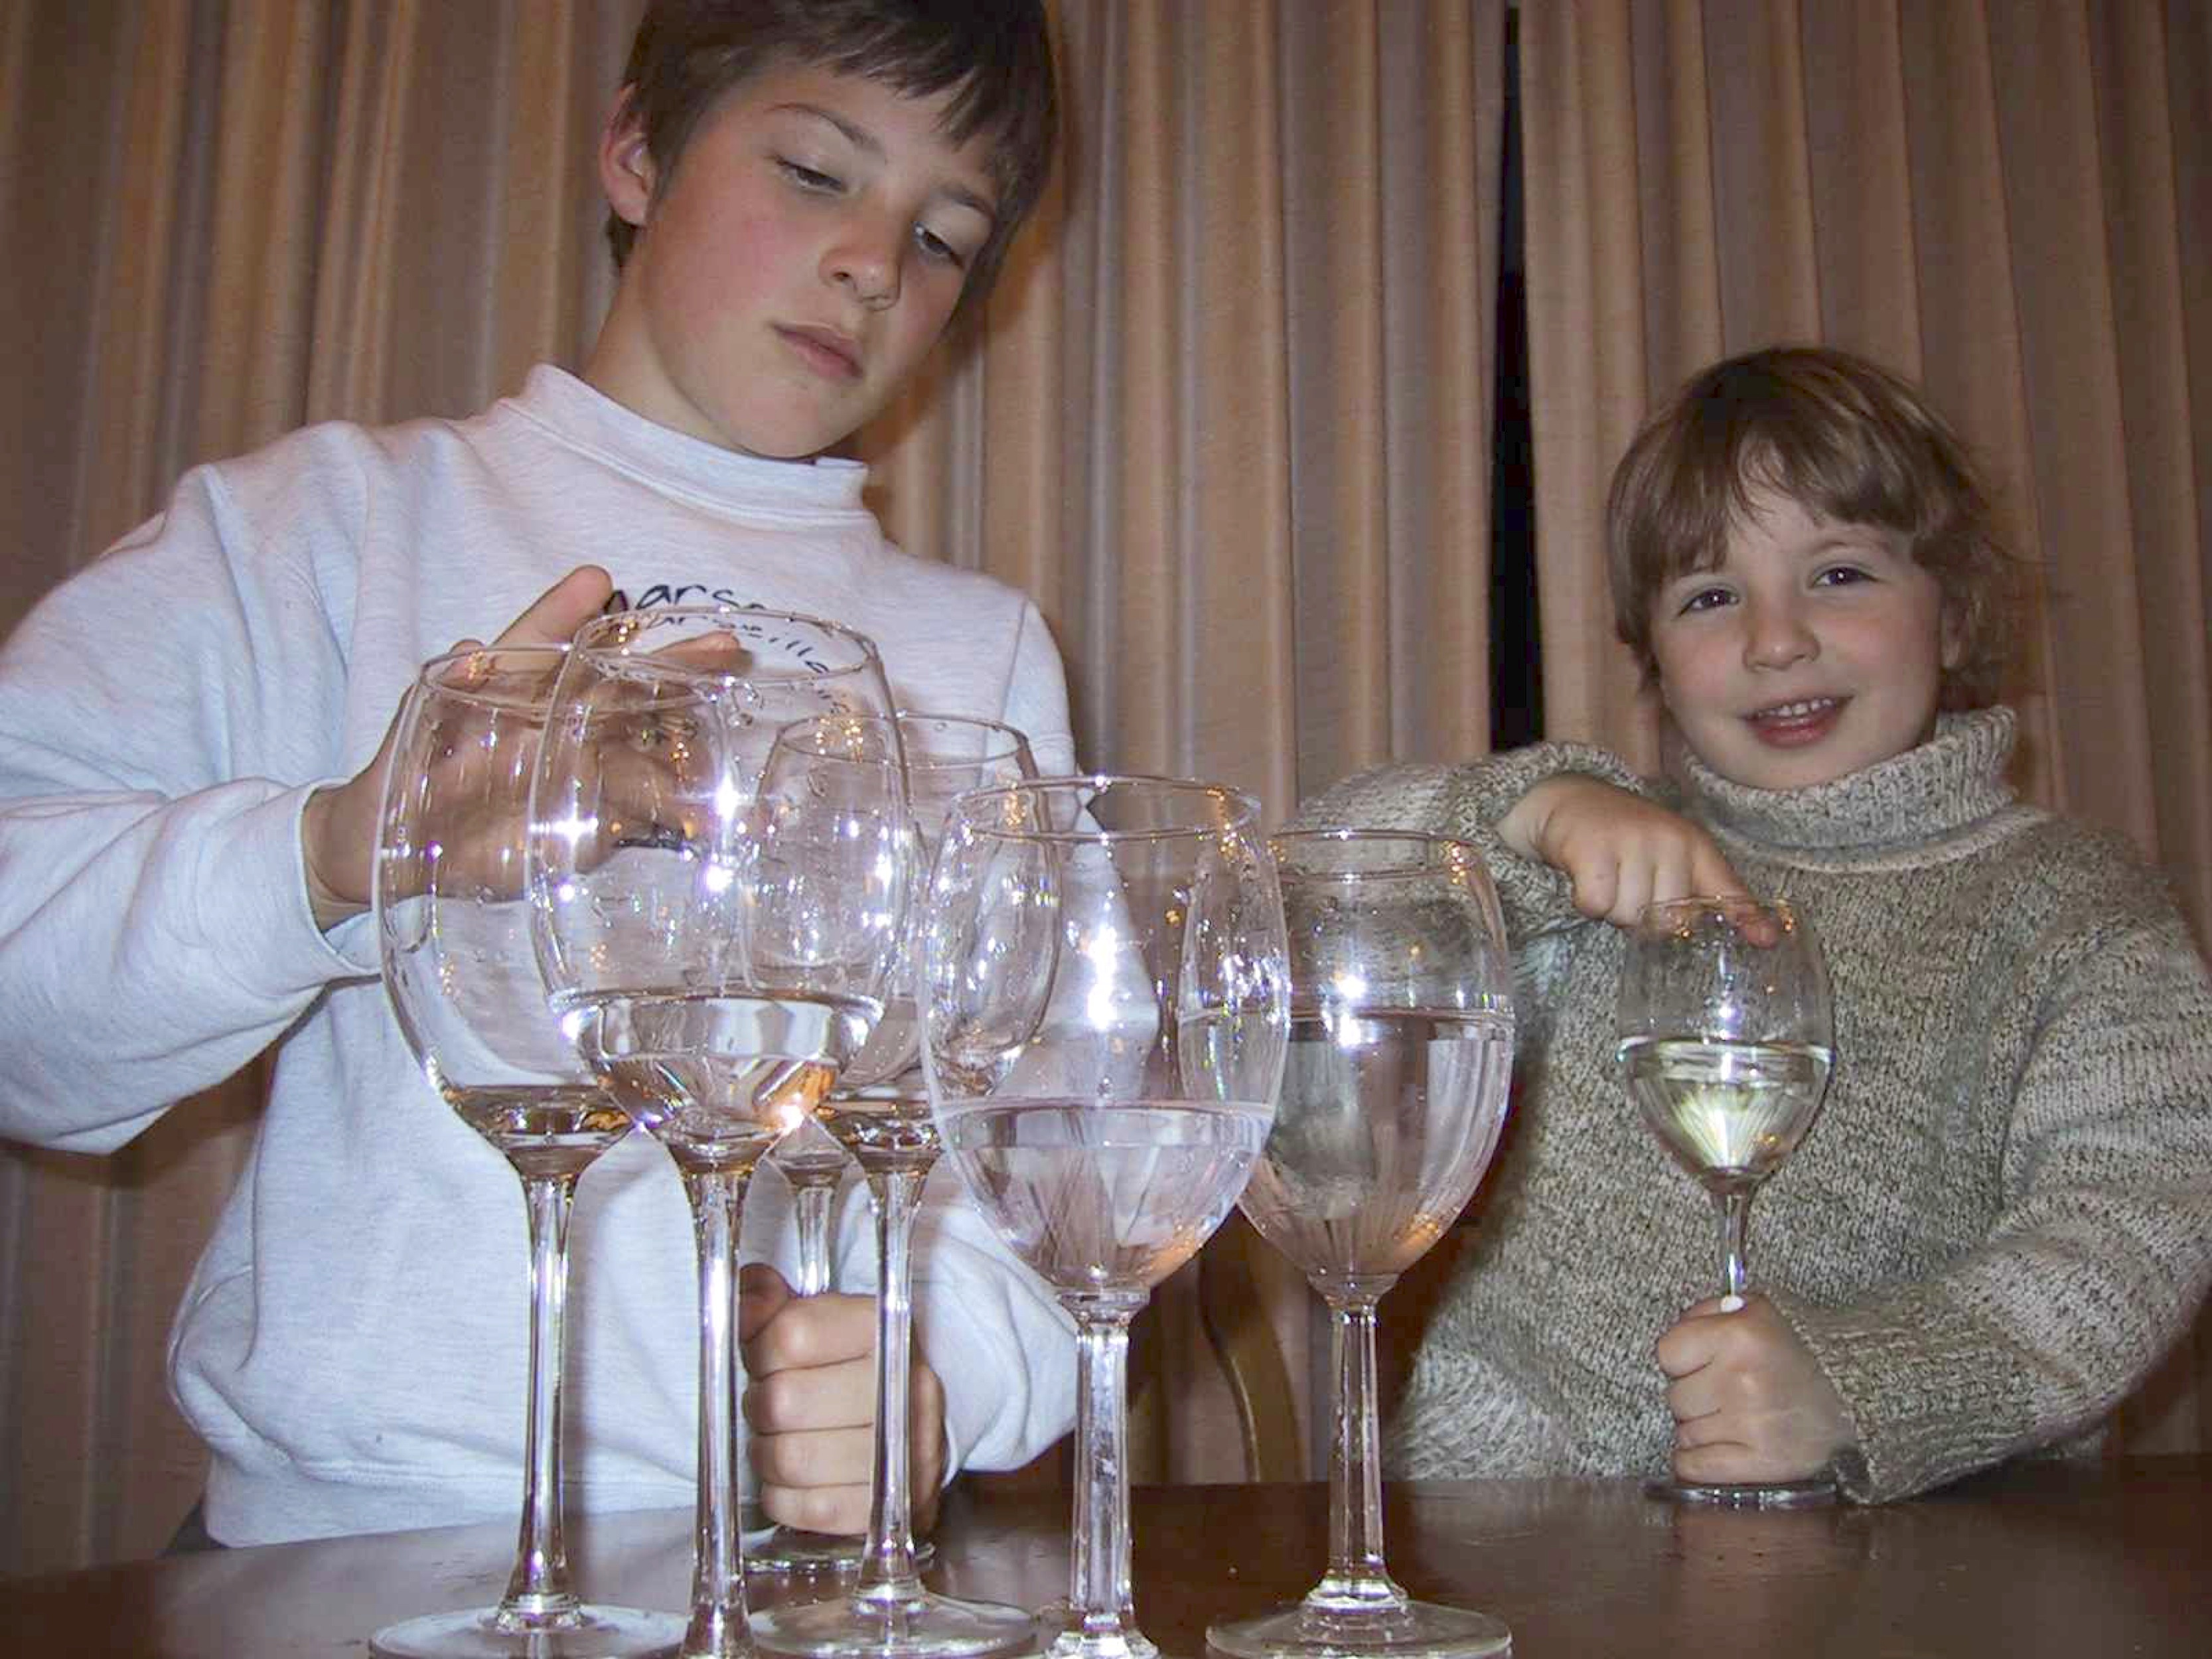
\includegraphics[width=7.8cm]{thomasfl.jpg}
\caption{Schematic of a gesture-sound interactive system, or ``movement sonification'' system}
  \label{Serafin:fig:2}
\end{figure}

\subsubsection{Modeling a Tibetan Bowl and a Glass Harmonica}

In \cite{Serafin:2002} we proposed a physical model of a Tibetan bowl implemented using banded waveguides  \cite{Essl:1999}. Banded waveguides are a particular case of waveguide networks in which each waveguide represents one strong resonance of the system. For a detailed description of banded waveguides, see \cite{Essl:2004}. The strong characteristic beatings of the instrument were implemented using detuned banded waveguides \cite{Serafin:2002a}. Considering the similarity of the structure of the Tibetan bowl and the glass harmonica, also the glass harmonica can be modeleled using banded waveguides. The two instruments are driven by the friction driven mechanism described in  \cite{Serafin:2004}.

\subsection{A Controller for Tibetan Bowl and Glass Harmonica}
The physical input parameters that control the excitation of a singing bowl (when bowed/rubbed with the playing stick) are the pressure of the stick against the surface of the bowl and the speed with which the stick travels around the bowl's edge. (The other features that affect the resonance of this instrument are related to the size, shape, and material qualities.)

In order to play a model of a singing bowl, a controller was developed called the HyperPuja  \cite{Young:2003a}. This interface was designed with minimal electronics, including a wireless RF transmitter, embedded inside the core of a traditional playing stick. The speed of the stick is measured using a small set of magnets adhered (not permanently) to the inside of a traditional Tibetan bowl and Hall sensors on the inside of the stick. (The time between peaks in the output of the Hall sensor indicated the speed with which the stick traverses the rim of the bowl.) Moreover accelerometers on the bowl stick for added control are inserted.

The pressure of the stick against the bowl was captured by a custom-made force sensitive resistor. The outside of the stick was wrapped in copper foil, over which was placed layer of thin conductive rubber, topped with a layer of copper mesh. The rubber is seen as a resistor, whose resistance decreases with increasing pressure. The sensor assembly was covered using a piece of chamois, similar to the thickness and texture of suede commonly used to wrap playing sticks. The implementation of this controller allows for easy control of Tibetan bowl models using normal playing techniques.

In addition, because the enhancement of the traditional instrument does not significantly impede its acoustic capabilities, it allows for electroacoustic performances combining the virtual bowl sound with the real bowl sound. Because of the great similarity between the glass harmonica and the Tibetan singing bowl models, we assert that the same controller may be used to play both.

\section{Musical Saw and Bowed Cymbal}

When an ordinary handsaw is bent into an S-shape, an interesting acoustical effect can occur. Tapping the blade of the saw reveals that beyond a certain critical degree of curvature, a very lightly damped vibration mode appears which is confined to the middle region of the S. This confined mode can be excited by a violin bow, to produce the pure sound of the musical saw.

The origins of the musical saw go back to the early 20th century, especially among the folk instrument community. Some important contributors to the development of the musical saw have been Leon and June Weaver. They also started playing the saw using a violin bow in a lap style, as shown in Figure~\ref{Serafin:fig:sawperf}.

\subsection{Modeling a Musical Saw}
\begin{figure}[t]
\centering
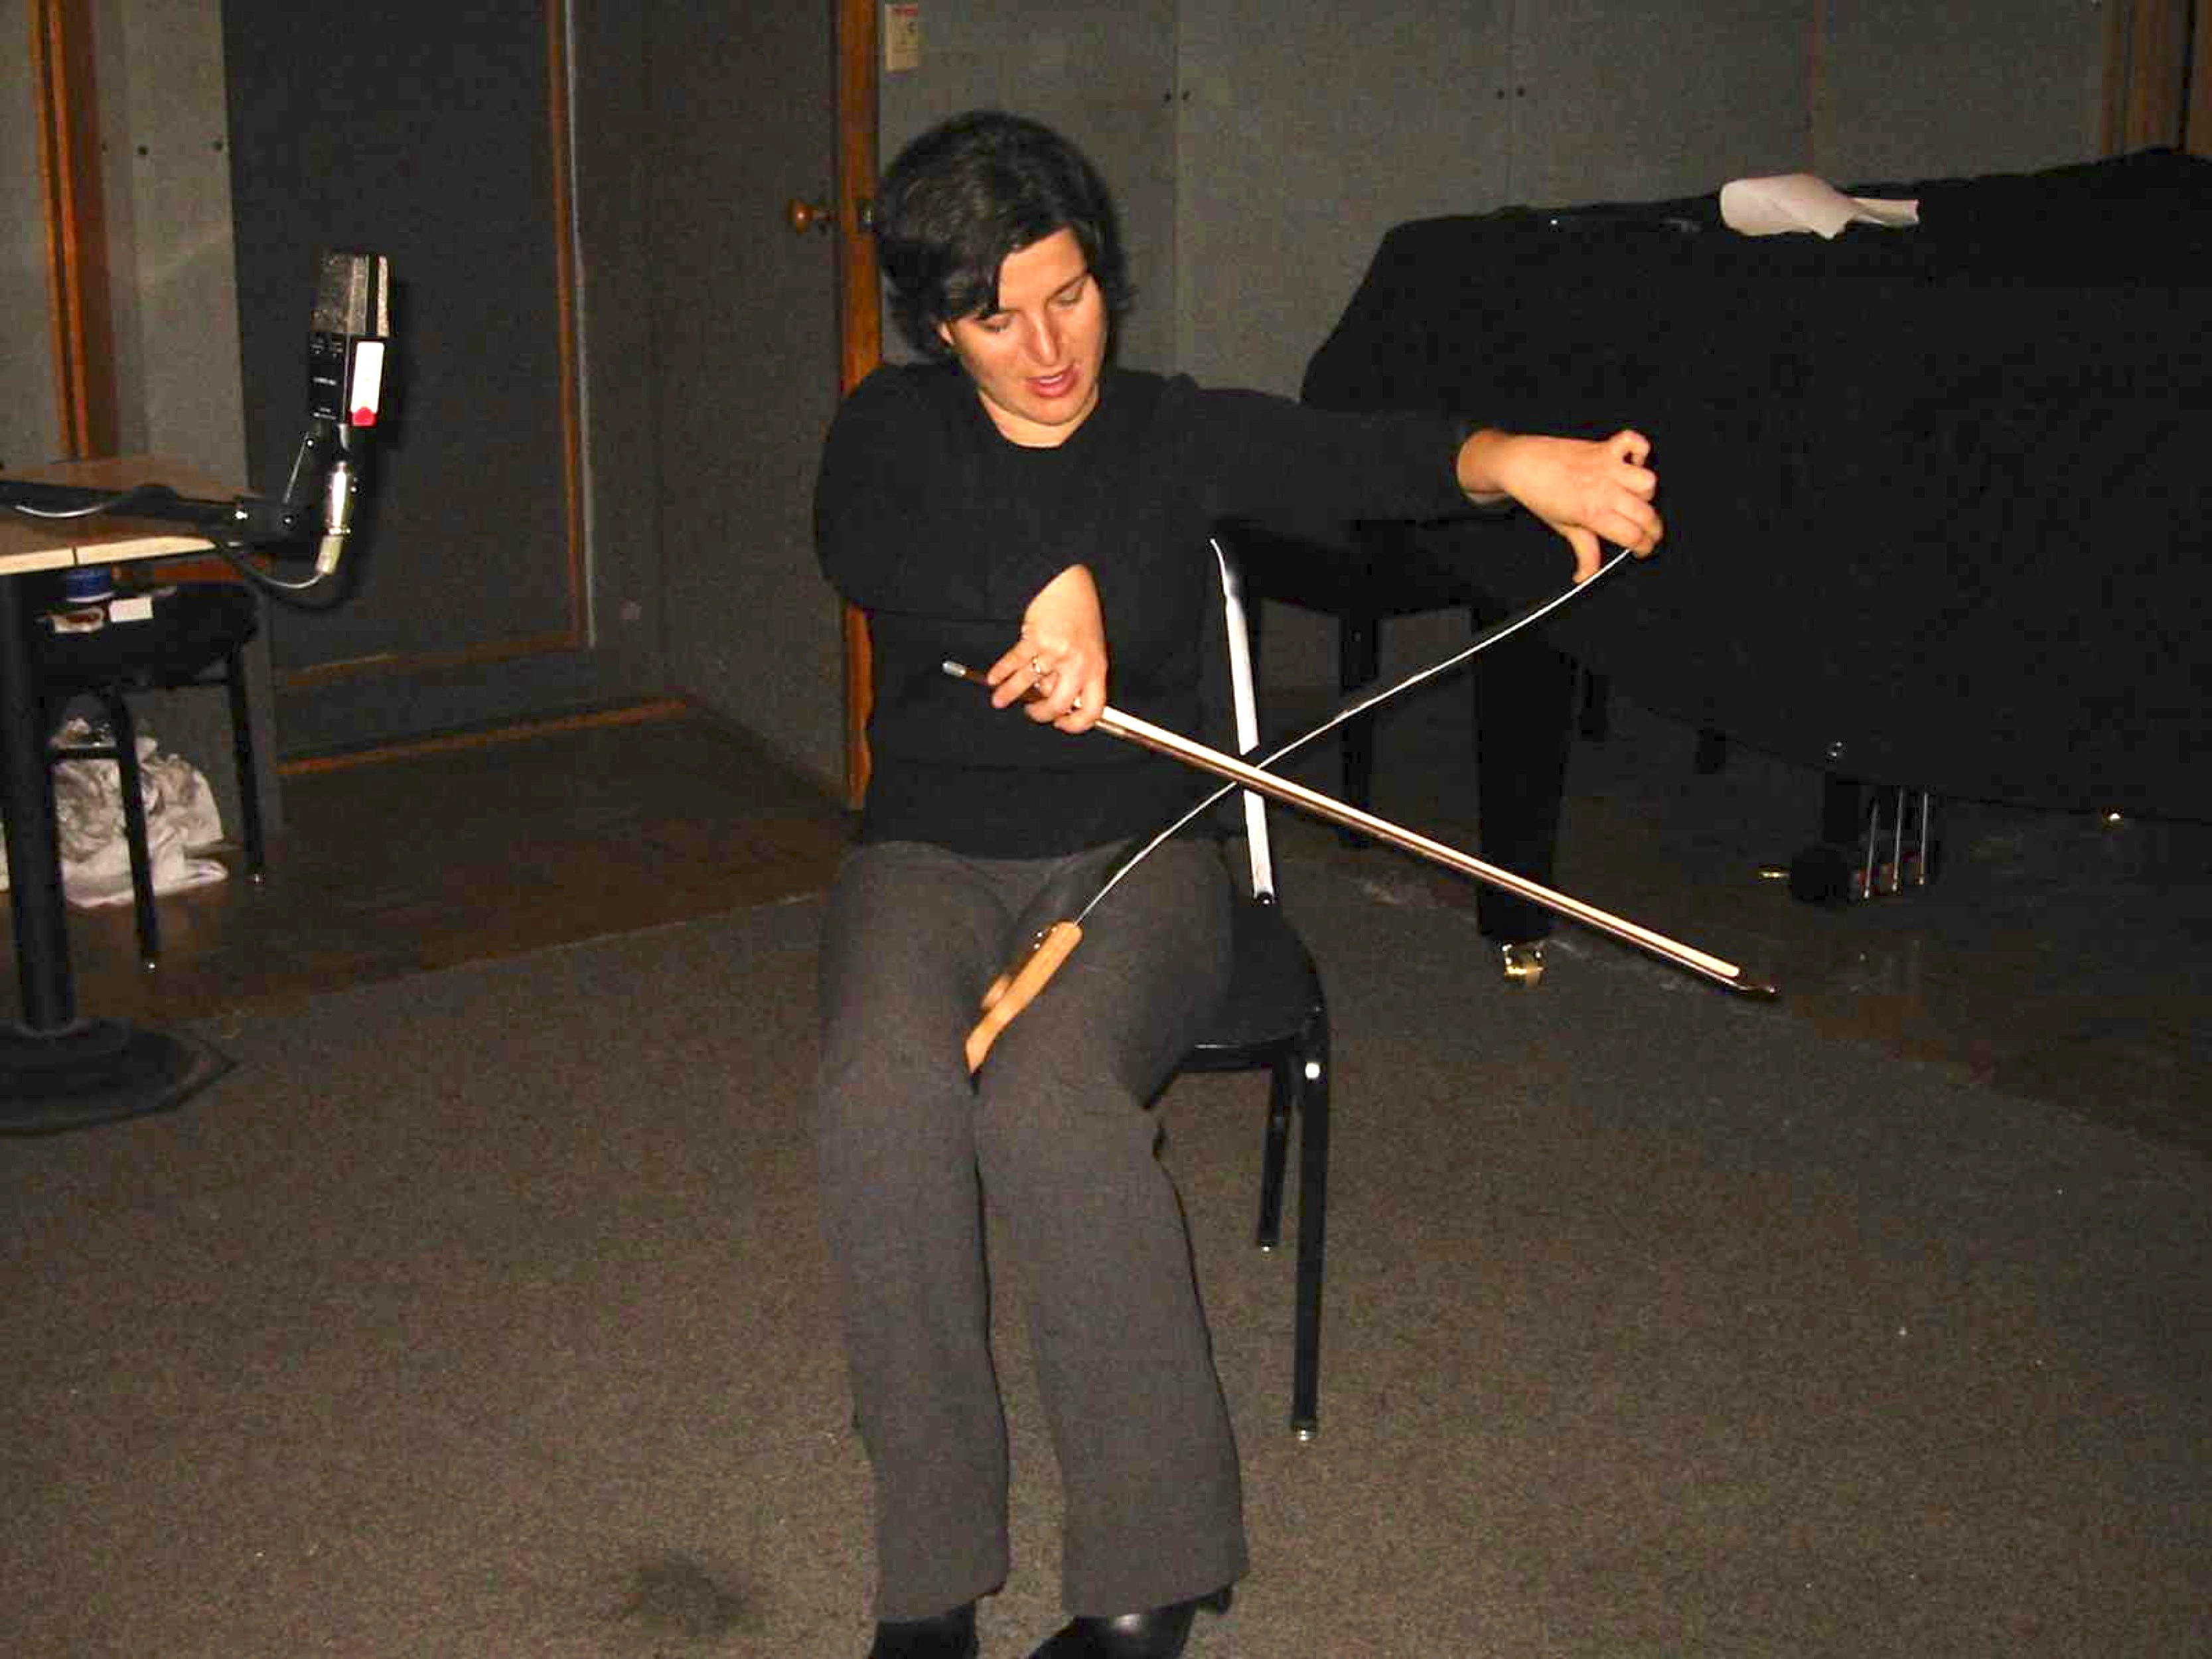
\includegraphics[width=\textwidth]{sawperf.jpg}
\caption{The musical saw.}
  \label{Serafin:fig:sawperf}
\end{figure}

In \cite{Serafin:2002} we proposed a physical model of a musical saw implemented using banded waveguides \cite{Essl:1999}. Given the simplicity of the spectrum of the musical saw, a single banded waveguide can be used to obtain a realistic simulation of the instrument.

\section{Bowed Cymbals}

As described in  \cite{Serafin:2004}, the vibration of a cymbal is very similar to the vibration of flat circular plates. While modes are clearly distinguishable at low frequencies, at high frequencies they often mix with one another. The nonlinear coupling between vibrational modes, moreover, is pretty strong, which makes many partials appear quickly in the spectrum. This is true no matter how the cymbal is excited.

In  \cite{Serafin:2004} an investigation of nonlinearities in cymbals is described. The results of exciting a cymbal with a sinusoidal shaker show that, while at low frequency the radiated sound is concentrated at the fundamental of the exciting frequency, increasing the amplitude increases also the relative levels of all the partials. At a critical excitation amplitude the spectrum develops a complete set of subharmonics, and transitions to fully chaotic behavior can appear. The mathematical problem of analyzing cymbal behavior in detail is rather complex. The frequency response of a bowed cymbal presents a large number of potentially active modes.

\subsection{Modeling Bowed Cymbal}
In order to simulate bowed cymbals and plates, in  \cite{Serafin:2001} we proposed a structure called banded waveguide mesh. The banded waveguide mesh is an extension to multiple dimensions of the banded waveguide in order to allow a real-time implementation. Low frequency modes are simulated using banded waveguides, while high frequency modes are simulated using a two dimensional waveguide mesh  \cite{Duyne:1993}.

\begin{figure}[t]
\centering
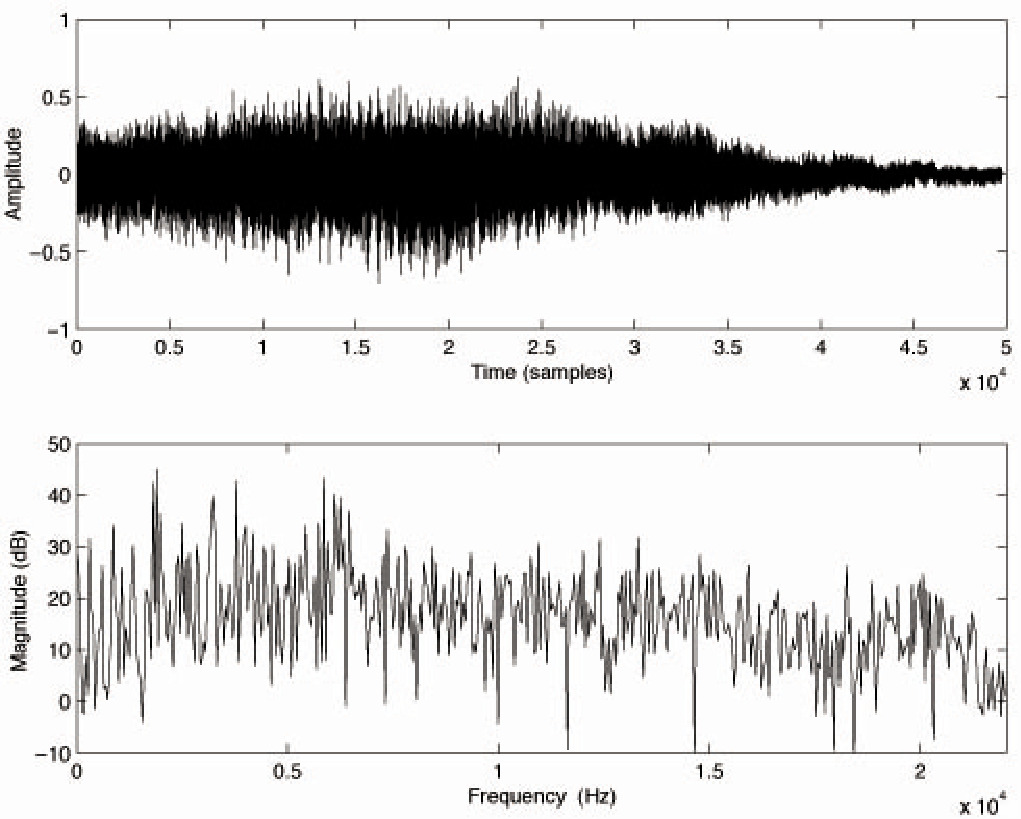
\includegraphics[width=\textwidth]{cymbal.pdf}
\caption{Time and frequency domain representation of a
bowed cymbal. Notice the rich spectrum.}
  \label{Serafin:fig:3}
\end{figure}


\subsection{A Controller for Musical Saw and Bowed Cymbal}

As with the Tibetan singing bowl, we sought a controller
for the musical saw and bowed cymbal that is as traditional in feel and appearance as possible. In order to play these models we used the bow controller as for the bowed string experiments in other recent work.

Primarily, we use the bow controller's capabilities of reflecting speed, using an electric field sensing technique, and force (as seen in the bending of the bow stick) as input parameters to the models. Like the other controller discussed, the implementation of the sensing elements here was done with great care to maintain playability and allow for typical playing techniques and styles.

Again, because the enhancements of the original acoustic interface do not impede the acoustic behaviours of the instrument, it is possible to provide performers with the ability to access both the real and the virtual instruments in the same performance, using the same interface. For a detailed description of the bow controller, see \cite{Young:2002a}.


\section{Toward a Generalized Friction Controller}

Though the two controllers discussed here offer many possibilities to performers due to their traditional feel, appearance, and function, it is legitimate to ask whether in many scenarios a less traditional interface may be more beneficial. Specifically, we are developing a general interface for the control of all friction-driven instrument models.

Such a device would likely share some of the physical qualities of a bow and playing stick, but having characteristics that imply different playing techniques. The challenges on the design of this device are due to the fact that friction sounds are produced in different ways such as perpendicular motion of the exciter on the resonator (like in the case of the bowed string and the musical saw), or circular motion (like in the Tibetan bowl and glass harmonica). We are currently experimenting with having a pressure sensor, a combination of different types of position sensors (Hall technique), strain/bend sensors like the ones used in the bow controller, accelerometers, and gyros for angular velocity. Such an instrument, however, will give composers and performers great possibilities to explore and extend the sound of friction.


\section{Conclusion}

We have presented several case studies of musical instruments that operate by means of a friction-based excitation mechanism much like that of a violin. We have described modelling techniques used to create their virtual instrument counterparts, as well as controllers that may be used to allow intuitive performances of them. Finally, we propose the creation of a generalized friction controller that could be used not only to play all of the virtual instruments highlighted in this paper, but also assist in the creation of hybrid electroacoustic instruments that utilize real-time physical models.

\section*{Author Commentary: About Generalized Friction Controllers}

\paragraph{Stefania Serafin and Diana Young}

This paper, exploring the concept of a generalized friction controller, reflects the work performed as part of our PhD dissertations. Stefania's dissertation, defended at the Centre for Computer Research in Music at Acoustics (CCRMA) at Stanford University in 2003 was entitled: ``The Sound of Friction: Real-time models, playability and musical applications.''  In this dissertation several real-time friction models for sound synthesis were presented, with applications to simulating bowed string instruments and also glass harmonicas, tibetan singing bowls, musical saws and other unusual friction-driven musical instruments. Diana's dissertation, completed in 2007 at Massachusetts Institute of Technology, was entitled: ``A Methodology for Investigation of Bowed String Performance Through Measurement of Violin Bowing Technique.'' As part of this work, Diana built the Hyperbow, a high-precision wireless sensing system, to measure violin bowing parameters.

The topics of our dissertations overlapped nicely, and when we met in 2002 at the CCRMA summer workshop on Physical Interaction Design for Music, we decided to collaborate. An obvious collaboration was to use Diana's Hyperbow controller to drive Stefania's bowed string physical models. The use of physical models in new interfaces for musical expression supports a natural interaction between performer and resulting sound, as the performer is given control of the physical parameters of the model in a manner that resembles the control of the real instrument counterpart. This is clear for the case of the Hyperbow, which is an augmented bow controller that naturally lends itself to the control of bowed string physical models, enabling any bowed string player to access to the expressive possibilities of virtual string instruments. This work has been published in several venues, such as the 2003 Symposium of Musical Acoustics \cite{Serafin:2003}, the 2003 edition of the New Interfaces for Musical Expression Conference \cite{Young:2003b}, and  the proceedings of the 2007 International Computer Music Conference \cite{Young:2007}. In addition to this body of work, the Hyperbow, once adapted for use with acoustic and electric cello, served as an integral part of a collaboration with composers and cellists at the Royal  Academy of Music, the focus of which was to further explore its expressive musical potential \cite{Young:2006}.  

The paper is mostly an overview of digital friction-driven musical instruments and their potential for natural control in expressive performances. In particular, we proposed several realistic gesture controllers to drive models of friction-driven instruments, such as tibetan singing bowls, musical saws and bowed cymbals. For controlling the Glass Harmonica and Tibetan singing bowl we suggest to use the HyperPuja \cite{Young:2003a}, a wireless controller in the form of a stick with embedded sensors hidden inside. For controlling the musical saw and bowed cymbals, we proposed the use of an augmented bow controller.

Writing this commentary, we realized it has been more than ten years since our collaboration, so it also gave us the opportunity to review recent work in the bowed string research community. While research on bowed string synthesis and control has continued to grow steadily, there has not been much significant progress in the development of realistic controllers for these virtual instruments that preserve traditional playing techniques. As bowed string enthusiasts, we still believe in the tremendous potential of this paradigm for musical expression. However, creating a faithful match between controller and model, e.g., of a violin, is challenging, especially given the high expectations for the traditional acoustic counterparts. 

Given the advances in sensor technology and wireless communication that have occurred since our last contributions, which pre-dated the smart phone revolution, we believe the time is right for serious re-investigation into controllers for bowed string physical models. In addition to the improved affordability and miniaturization of electronics, materials and access to fabrication tools have also increased. In the case of bowed strings, we believe it is now possible to dramatically improve upon the sensing system of the Hyperbow by making it more precise, while also streamlining its ergonomics by embedding it within the construct of a traditional carbon fiber bow. Similarly, the model could be made to run locally within the body of the violin controller, rather than relying on an external computer. Such advances would further support the relationship between the player and instrument, and the development of a new repertoire for virtual strings. 



\section*{Expert Commentary: Some Thoughts on Friction and Physicality Within Past and for Future NIME Research}

\paragraph{Lauren Hayes}

Stefania Serafin and Diana Young present a paper which identifies friction as the force that is employed within the excitation mechanism of four unique types of acoustic instrument. They recognise that each instrument sounds as the result of a hard object being rubbed on part of the instrument's surface. Rather than focussing on the commonly modelled bowed string, they pick four instruments with a diverse sonic palette: the musical saw, Tibetan singing bow, glass harmonica, and bowed cymbal. The Tibetan singing bowl, for example, needs to be activated by a suede-clad stick that is moved in circles around its inner rim.

The authors consolidate a significant body of research within this short paper by describing their designs of both the physical models of these instruments, as well as devices that can be used to play them. For example, Serafin's contribution to banded waveguide synthesis techniques \cite{Essl:2004} is employed to establish a physical model of a Tibetan bowl. Each prominent resonance within the bowl's ringing sound is represented by a waveguide, and various beating effects can be achieved by subsequently detuning these. Similarly, Young's Hyperbow interface, which she has developed and revised extensively over many years, is used to play models of a musical saw and bowed cymbal. 

The crux of Serafin and Young's short paper lies in the authors' abilities to observe commonalities between the playing mechanisms of these unique instruments. They ask whether a new type of interface might offer a performer playing physical models of the acoustic versions further possibilities for exploration. They propose a generalised friction controller which would allow for combinations of gestures such as circular movements (stick), as well as back-and-forth motions (bow). This goal is realised in later work \cite{Gelineck:2010}, in which a two-dimensional friction device is built and included as part of a larger instrument, PHYSMISM, which is designed to play and combine physical models.

The authors emphasise physicality as a key consideration for the design of NIMEs. They suggest that performer--instrument interaction needs to be  ``natural and instinctive,'' and they talk about achieving ``easy intuitive control.'' The notion of control is problematic when discussing musical instruments. As I have written previously, hybrid pianos, just as acoustic pianos, are played rather than controlled \cite{Hayes:2013}. When performing with systems that are, for example, unpredictable in part, it may be precisely the lack of control that allows us to fully engage with the instrument. Creative possibilities may be thrown our way, as we attempt to navigate through a performance. Similarly, it is important to carefully consider whether new instruments should be easy to play when developing a design philosophy.

Serafin and Young clearly recognise the importance of the relationship between performers and instruments. Related work involving PHYSMISM, of which the friction controller is an integral part, discusses how the physical interface might go beyond simply improving the level of intimacy that a performer has with their instrument by allowing for creative exploration through its use \cite{Gelineck:2010}. This is interesting in two ways. Firstly, as PHYSMISM would allow physical models to be played in ways that their acoustic counterparts could not be played, it could lead to potential new sounds. Secondly, while the feel of and sensations involved in playing an instrument are crucial to a performer \cite{Essl:2006}, they can also impact the compositional or inventive aspect of musical creativity. In my own work, I have employed vibrotactile feedback not only to aid my performances through enhanced haptic sensation, but also to allow me to access how my music actually feels during the process of its creation \cite{Hayes:2013}. The act of composing becomes an embodied experience itself.

Turning back to performers, Young's Hyperbow has been used by professional violinists, among others, in various performance settings \cite{Young:2002a}. However, in reviewing the literature related to this paper, what seems to be missing is the voice of the performers who have worked with these instruments. Summarising comments on observational studies have their place, but in-depth descriptions of practice and ethnographic inquiry into performances, rehearsals, and recordings made using these instruments can only help to legitimise the importance of this work. It is easy to imagine how performers and composers might benefit from being able to explore friction within a NIME and it would be helpful to read more about this too. As with most NIME research, we need more long-term accounts from those who regularly play, perform with, or workshop these often under-explored instruments.

